\documentclass[11pt]{article}
\usepackage[margin=1in]{geometry}
\usepackage{amsmath, amssymb}
\usepackage{graphicx}
\usepackage{booktabs}
\usepackage{hyperref}
\usepackage{authblk}
\usepackage{xcolor}

\title{Credit Card Fraud Detection via a Heterogeneous Stacking Ensemble of Supervised and Unsupervised Models}

\author[1]{Joe Tesoriero\thanks{\texttt{joseph.tesoriero@ucdenver.edu}}}
\author[1]{Ronald Yu\thanks{\texttt{ronald.yu@ucdenver.edu}}}
\author[1]{Tejal Jadhav\thanks{\texttt{tejalvilas.jadhav@ucdenver.edu}}}
\affil[1]{Department of Computer Science and Engineering, University of Colorado Denver \\ CSCI-5931: Deep Learning}
\date{May 2026}

\begin{document}
\maketitle

\begin{abstract}
This project tests whether a stacked ensemble that combines a supervised neural network, supervised gradient boosting (XGBoost), and two unsupervised anomaly detectors (autoencoder, isolation forest) can outperform any single base model on credit card fraud detection. The predictions from each base model are combined through a learned meta-classifier using out-of-fold stacking, which prevents label leakage. We evaluate six meta-learner families on two datasets (Kaggle CreditCard and BankSim) and report bootstrap 95\% confidence intervals on F1 and AUC-PR. The results show that the ensemble matches but does not statistically beat a well-tuned standalone XGBoost on either dataset. The most defensible benefit of the ensemble is robustness. The meta-learner correctly down-weights weak base models (autoencoder on CreditCard, isolation forest on both datasets) instead of being dragged down by them.
\end{abstract}

% ========================================================
\section{Problem Statement}
% ========================================================

Credit card fraud detection is a binary classification problem on highly imbalanced tabular data. Given a transaction described by a feature vector $\mathbf{x} \in \mathbb{R}^d$, the model must output a probability $\hat{y} \in [0,1]$ that the transaction is fraudulent. Fraud is rare. In the Kaggle CreditCard dataset, only 0.17\% of transactions are fraud. In BankSim, 1.2\% are fraud. Models must balance two competing costs. Missing fraud (false negatives) results in financial loss to the cardholder or issuer. Flagging legitimate transactions (false positives) damages user trust and operational throughput.

The research question for this project is: does combining supervised and unsupervised learners under a stacked meta-classifier provide a statistically significant improvement over the best single base model?

% ========================================================
\section{Motivation}
% ========================================================

\subsection{Application importance}
Card fraud is a large and growing problem, especially as more transactions move online. Even small improvements in fraud detection precision or recall translate to real savings, while incorrectly blocked transactions cause customer churn. Industrial fraud detection systems are almost always ensembles in practice, but the published literature is fragmented across paradigms (supervised vs. unsupervised), and the ensembling approaches in those papers are often ad-hoc rather than principled.

\subsection{Gap addressed}
Prior work has either (i) trained multiple supervised classifiers and reported their individual scores side by side without a learned combiner~\cite{alarfaj2022}, or (ii) combined two unsupervised methods in a fixed (non-learned) configuration~\cite{pumsirirat2018}. We were unable to find published work that uses a learned meta-classifier to combine both supervised and unsupervised paradigms via out-of-fold stacking, with a systematic comparison across meta-learner families. This project addresses that gap.

\subsection{Ethical considerations}
There are three ethical concerns that informed our design and reporting:

\begin{enumerate}
    \item \textbf{Demographic fairness.} BankSim includes demographic features (age bucket, gender). A model that achieves high overall F1 by disproportionately flagging transactions from certain demographic groups would be unfair. We did not perform a full subgroup fairness audit in this report, but flag it as required future work before any deployment.
    \item \textbf{False positive cost asymmetry.} A blocked legitimate transaction can cause real harm (stranded traveler, missed bill). The cost-sensitive threshold tuning experiment in this project models this asymmetry ($10 \times \text{FN} + 1 \times \text{FP}$), but the cost ratio itself is a value judgment that should be set by domain experts, not data scientists.
    \item \textbf{Honest reporting under small sample uncertainty.} The CreditCard test set contains only 71 fraud cases. A single misclassification moves F1 by about 0.013. We compute bootstrap confidence intervals on all reported metrics, and we refuse to claim model A is ``better than'' model B when the intervals overlap. The broader fraud detection literature is full of point-estimate comparisons that do not survive this scrutiny.
\end{enumerate}

% ========================================================
\section{Related Works}
% ========================================================

\paragraph{Autoencoders for fraud anomaly detection.}
Pumsirirat \& Yan~\cite{pumsirirat2018} train a deep autoencoder and a restricted Boltzmann machine on normal transactions only, then flag high reconstruction error as fraud. Both components are unsupervised, and their combination is a fixed rule rather than a learned one.

\paragraph{Comparative classifier studies.}
Alarfaj et al.~\cite{alarfaj2022} benchmark many classifiers (logistic regression, decision trees, SVMs, neural networks) individually on the Kaggle CreditCard dataset. There is no learned ensembling in their work.

\paragraph{Tabular deep learning vs. tree-based methods.}
Grinsztajn et al.~\cite{grinsztajn2022} show that on a broad benchmark of tabular tasks, gradient-boosted trees consistently outperform deep neural networks, even with extensive tuning. This finding is highly relevant to our results.

\paragraph{Stacked generalization.}
Wolpert~\cite{wolpert1992stacking} introduced stacking with out-of-fold predictions as a way to combine base learners without label leakage. We follow this protocol for the supervised members of our stack.

% ========================================================
\section{Methods}
% ========================================================

\subsection{Architecture overview}
The pipeline has two layers, shown in Figure~\ref{fig:pipeline}:

\begin{enumerate}
    \item \textbf{Base layer (4 models).} A feedforward neural network (FFN) and XGBoost are trained as supervised classifiers on the labeled training set. An autoencoder (AE) and isolation forest (IF) are trained on the normal-only subset and produce continuous anomaly scores.
    \item \textbf{Meta layer.} For each training sample, we form a 4-dimensional feature vector $[\hat{p}_{\text{FFN}}, \hat{p}_{\text{XGB}}, s_{\text{AE}}, s_{\text{IF}}]$ and train a meta-classifier to produce the final fraud probability.
\end{enumerate}

\begin{figure}[h]
\centering
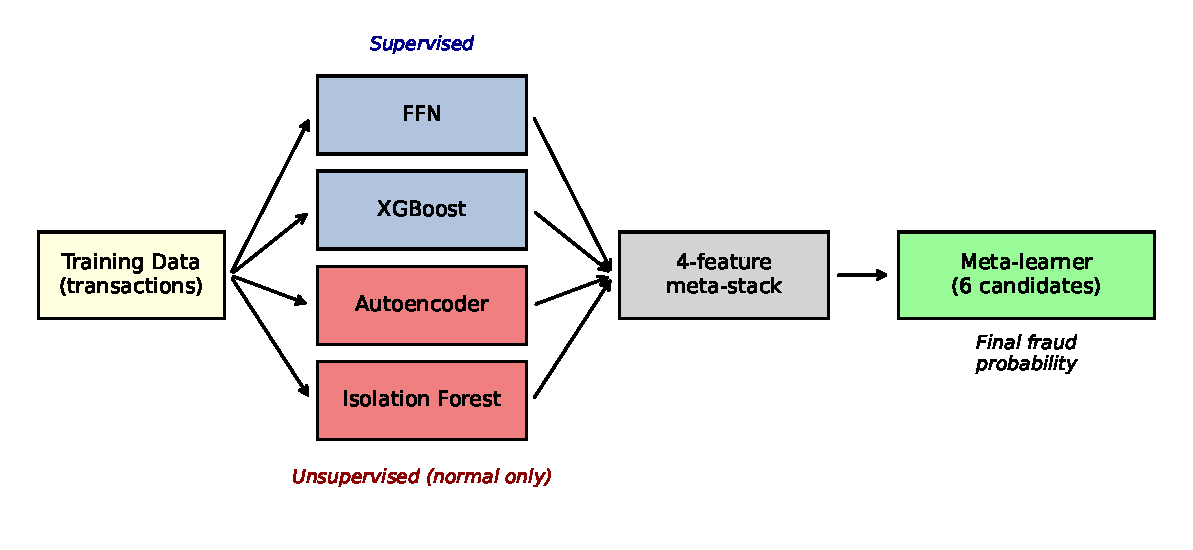
\includegraphics[width=0.95\textwidth]{figures/pipeline_diagram.pdf}
\caption{The stacking pipeline. Four base models produce per-transaction outputs that form a 4-feature meta-stack, which is then classified by one of six meta-learners.}
\label{fig:pipeline}
\end{figure}

\subsection{Out-of-fold stacking}
To avoid label leakage, the supervised base models' meta-features on the training set come from 5-fold out-of-fold (OOF) predictions. For each fold, the FFN and XGBoost are trained on the other four folds and used to predict the held-out fold. This ensures that every training sample has a prediction generated by a model that did not see that sample's label. The unsupervised models (AE, IF) have no label leakage by construction since they never see labels.

\subsection{Base model hyperparameters}
All base model hyperparameters were tuned via random search, and the resulting configurations are loaded at runtime from CSV files:
\begin{itemize}
    \item FFN: hidden layers $[256, 128, 64]$, dropout 0.35, Adam ($\eta = 0.0098$, weight decay $3\times 10^{-4}$), batch size 128.
    \item XGBoost: 400 trees, max depth 8, learning rate 0.21, $\texttt{scale\_pos\_weight}=\frac{|\text{neg}|}{|\text{pos}|}$.
    \item Autoencoder: encoder $[128, 64, 32, 16]$, Adam ($\eta=0.001$), batch size 256.
    \item Isolation Forest: 500 estimators, contamination 0.003.
\end{itemize}

\subsection{Meta-learner candidates}
We compare six meta-learners: Logistic Regression (linear baseline), Random Forest, Gradient Boosting (GBM), RBF-kernel SVM, MLP, and AdaBoost. The SVM is fit on a stratified 20{,}000-row subsample because the full $\mathcal{O}(n^2)$ kernel fit is too slow at our training set size.

\subsection{Evaluation protocol}
Datasets are split 70/15/15 (train/val/test), stratified by label. The decision threshold for each model is chosen by sweeping $[0.01, 0.99]$ on the validation set to maximize F1. That threshold is then applied to the test set. We report F1, precision, recall, and AUC-PR. To quantify uncertainty, we compute 95\% bootstrap confidence intervals (1{,}000 resamples with replacement) for F1 and AUC-PR on each test set.

% ========================================================
\section{Experiments and Results}
% ========================================================

\subsection{Datasets}
\begin{itemize}
    \item \textbf{CreditCard} (Kaggle, ULB): 284,807 transactions, 492 fraud (0.17\%). Features V1 through V28 are PCA-transformed (anonymized). Time and Amount are raw.
    \item \textbf{BankSim} (Kaggle, ealaxi): 594,643 transactions, 7,200 fraud (1.2\%). Features are interpretable: step, age bucket, gender, merchant category, amount.
\end{itemize}

\subsection{Headline results}

Table~\ref{tab:cc} shows F1 and AUC-PR with 95\% CIs on CreditCard. Table~\ref{tab:bs} shows the same on BankSim.

\begin{table}[h]
\centering
\caption{CreditCard test set results (71 fraud cases). Bootstrap 95\% CIs in brackets.}
\label{tab:cc}
\small
\begin{tabular}{lll}
\toprule
Model & F1 [95\% CI] & AUC-PR [95\% CI] \\
\midrule
FFN              & 0.786 [0.694, 0.857] & 0.701 [0.574, 0.818] \\
XGBoost          & 0.835 [0.755, 0.903] & 0.816 [0.725, 0.901] \\
Autoencoder      & 0.198 [0.154, 0.244] & 0.428 [0.310, 0.556] \\
Isolation Forest & 0.199 [0.141, 0.253] & 0.130 [0.086, 0.203] \\
Meta-LR          & 0.803 [0.720, 0.874] & \textbf{0.820} [0.729, 0.904] \\
Meta-RF          & 0.794 [0.711, 0.870] & 0.789 [0.694, 0.880] \\
Meta-GBM         & 0.064 [0.000, 0.141] & 0.019 [0.004, 0.064] \\
Meta-SVM         & 0.326 [0.261, 0.390] & 0.122 [0.090, 0.176] \\
Meta-MLP         & 0.831 [0.752, 0.900] & 0.803 [0.701, 0.893] \\
Meta-AdaBoost    & \textbf{0.844} [0.769, 0.909] & 0.773 [0.669, 0.873] \\
\bottomrule
\end{tabular}
\end{table}

\begin{table}[h]
\centering
\caption{BankSim test set results (1,080 fraud cases). Bootstrap 95\% CIs in brackets.}
\label{tab:bs}
\small
\begin{tabular}{lll}
\toprule
Model & F1 [95\% CI] & AUC-PR [95\% CI] \\
\midrule
FFN              & 0.720 [0.696, 0.740] & 0.766 [0.740, 0.791] \\
XGBoost          & 0.718 [0.694, 0.742] & 0.772 [0.749, 0.795] \\
Autoencoder      & 0.669 [0.640, 0.693] & 0.678 [0.649, 0.705] \\
Isolation Forest & 0.295 [0.273, 0.319] & 0.218 [0.198, 0.242] \\
Meta-LR          & 0.715 [0.692, 0.737] & 0.770 [0.747, 0.793] \\
Meta-RF          & 0.730 [0.705, 0.751] & 0.786 [0.763, 0.807] \\
Meta-GBM         & \textbf{0.732} [0.709, 0.755] & \textbf{0.803} [0.782, 0.824] \\
Meta-SVM         & 0.466 [0.439, 0.493] & 0.407 [0.379, 0.440] \\
Meta-MLP         & 0.732 [0.708, 0.754] & 0.785 [0.761, 0.808] \\
Meta-AdaBoost    & 0.732 [0.709, 0.753] & 0.766 [0.743, 0.789] \\
\bottomrule
\end{tabular}
\end{table}

\subsection{Statistical significance}
On CreditCard, the best meta-learner (Meta-AdaBoost, F1 = 0.844) has a confidence interval that almost entirely contains the standalone XGBoost interval (F1 = 0.835). The ensemble does not statistically beat XGBoost. On BankSim, the best meta-learner (Meta-GBM, F1 = 0.732) achieves a tighter CI thanks to the larger fraud count, but the interval still overlaps XGBoost's by a small margin. The difference is suggestive but not significant at $\alpha=0.05$. Figure~\ref{fig:forest} shows the F1 forest plot for both datasets.

\begin{figure}[h]
\centering
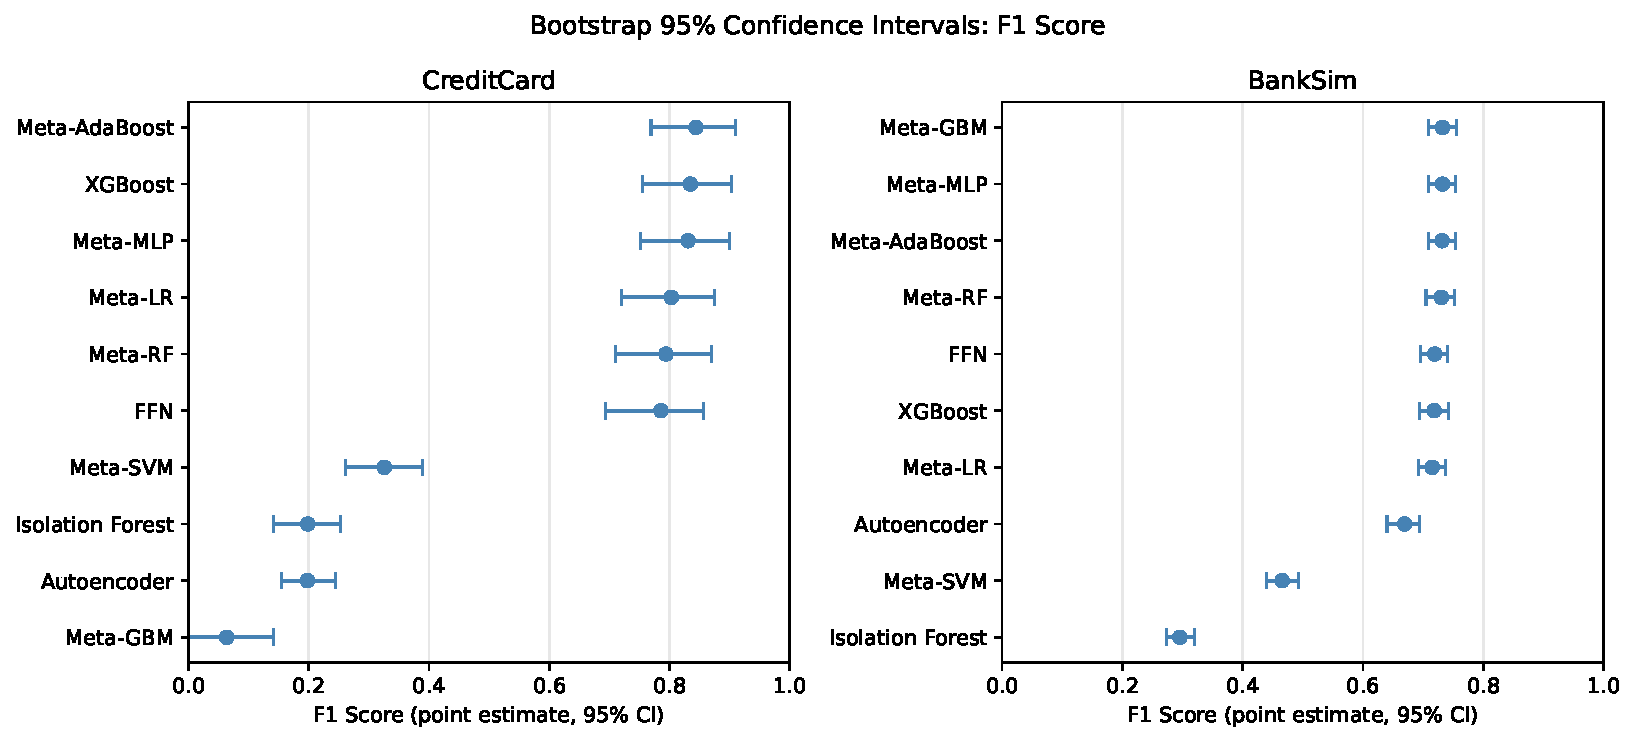
\includegraphics[width=\textwidth]{figures/forest_f1.pdf}
\caption{Bootstrap 95\% confidence intervals on F1 score for all models. CreditCard CIs are much wider than BankSim's because the CreditCard test set contains only 71 fraud cases. On both datasets, the top group of models overlap each other heavily, meaning the apparent ranking within that group is not statistically reliable.}
\label{fig:forest}
\end{figure}

\subsection{Cross-dataset comparison}
Figure~\ref{fig:cross} compares F1 and AUC-PR across both datasets. The ranking is broadly consistent (XGBoost and the top meta-learners cluster at the top, while Meta-SVM and Isolation Forest are at the bottom on both datasets), with two exceptions worth noting. Meta-GBM is the best meta-learner on BankSim but completely fails on CreditCard. The autoencoder is the inverse: weak on CreditCard but competitive on BankSim.

\begin{figure}[h]
\centering
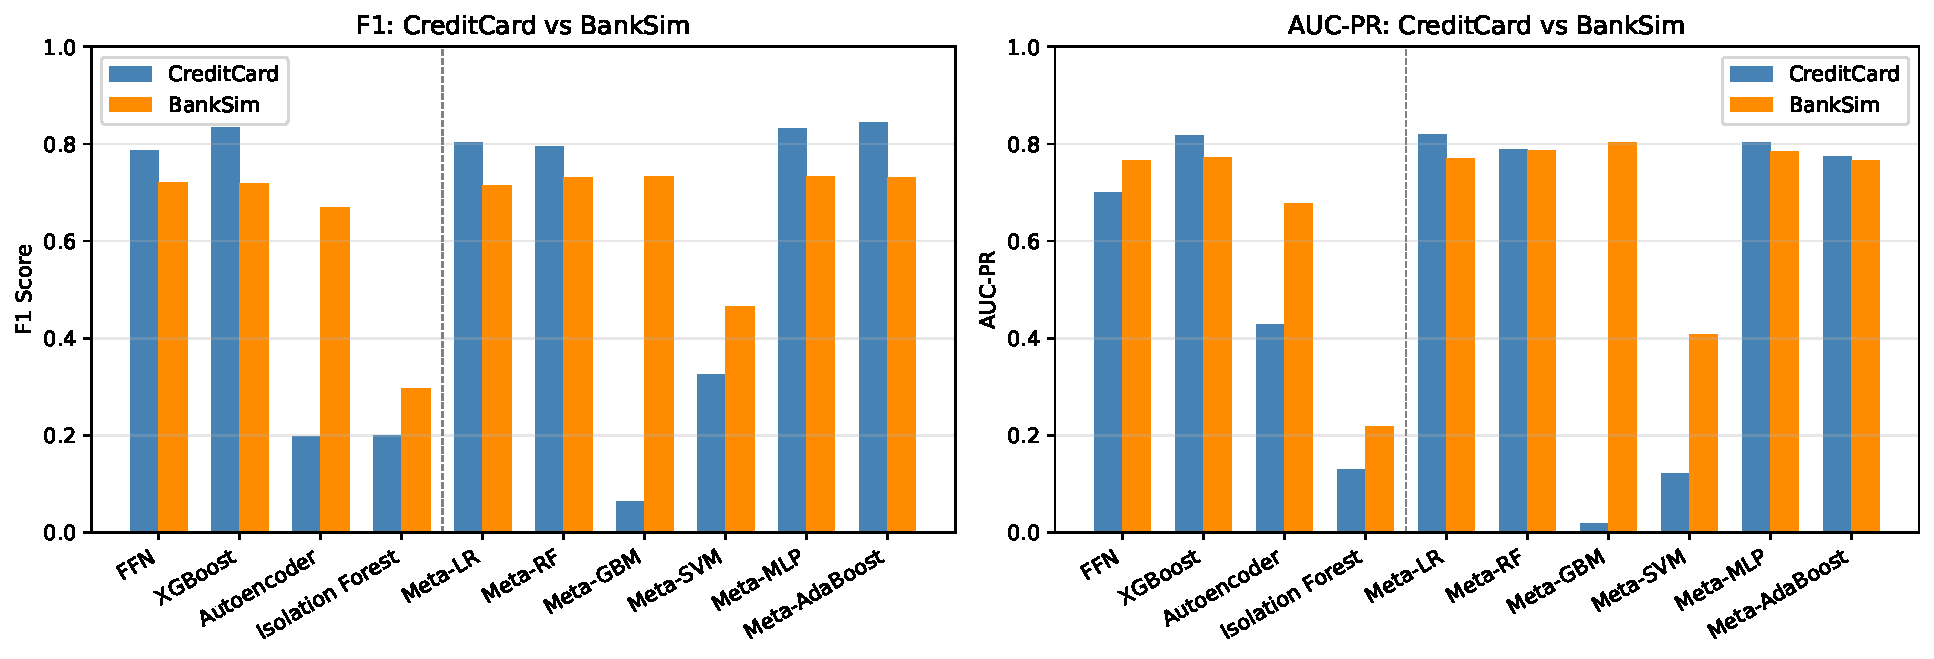
\includegraphics[width=\textwidth]{figures/cross_dataset_comparison.pdf}
\caption{F1 and AUC-PR for all 10 models on both datasets. The vertical dashed line separates base models (left) from meta-learners (right).}
\label{fig:cross}
\end{figure}

\subsection{Deep learning vs. gradient boosting}
On CreditCard, XGBoost (F1 = 0.835) outperforms the FFN (F1 = 0.786), though the gap of 0.049 falls within the overlapping confidence intervals, making the difference statistically ambiguous on this small test set. On BankSim, the two are statistically tied (FFN 0.720, XGB 0.718). This is consistent with Grinsztajn et al.~\cite{grinsztajn2022}: tree-based methods dominate on tabular data, especially when features are already preprocessed (PCA-transformed in CreditCard) and there is little hierarchical structure for an MLP to learn.

\subsection{Unsupervised behaviour is dataset dependent}
The autoencoder achieves F1 = 0.198 on CreditCard but F1 = 0.669 on BankSim. That is a 3.4$\times$ difference. The reason is feature semantics. CreditCard's PCA-transformed features are mean-centered and decorrelated, which removes the structure an AE would otherwise reconstruct. BankSim's raw categorical and amount features have meaningful ``normal-behaviour'' patterns. This suggests AE-based anomaly detection is appropriate only when the input features carry semantic structure.

\subsection{Meta-GBM collapse on CreditCard}
Meta-GBM achieves the best result on BankSim (F1 = 0.732), but it completely fails on CreditCard (F1 = 0.064). The very small CreditCard meta-training fraud count (331 cases over a 4-dimensional input) likely allows Meta-GBM to overfit a degenerate split rule. Stronger regularization or fewer estimators would likely recover performance.

% ========================================================
\section{Limitations}
% ========================================================

\begin{enumerate}
    \item \textbf{Statistical underpower on CreditCard.} With only 71 fraud cases in the test set, the bootstrap CIs are wide ($\sim 0.15$) and fine-grained model comparisons are not meaningful. This is a property of the dataset, not of our methodology.
    \item \textbf{BankSim is synthetic.} BankSim is a simulation, not real transactions. Patterns learned here may not transfer to production fraud streams.
    \item \textbf{Meta-learner hyperparameters are not tuned.} Base-model hyperparameters were tuned via random search. The six meta-learners use sklearn defaults (with adjustments only for class balance and reproducibility). A meta-learner hyperparameter sweep could change rankings, particularly for Meta-GBM and Meta-SVM.
    \item \textbf{No subgroup fairness audit.} BankSim contains demographic features (age, gender). We did not measure whether model performance is equitable across these subgroups. Production deployment would require this audit.
    \item \textbf{AE/IF train-data asymmetry.} Supervised base models use OOF predictions on the train set as meta-features (no leakage). The unsupervised models are trained on all normal training rows, then scored on the same training set. This is a technical leakage source (in-sample reconstruction for normal samples), but it is standard in one-class anomaly stacking and matches prior work.
    \item \textbf{Calibration not addressed.} AE/IF anomaly scores are converted to $[0,1]$ via sigmoid of standardized values. This is not a proper probability calibration in the Platt or isotonic sense. The meta-learner partially compensates, but a properly calibrated AE/IF probability stream could change results.
    \item \textbf{Graph structure unused.} BankSimNET adds customer to merchant graph edges to BankSim, which enables GNN approaches. We do not exploit this. Relational fraud patterns are left for future work.
\end{enumerate}

% ========================================================
\section{Conclusion}
% ========================================================

A heterogeneous stack combining supervised deep learning, supervised gradient boosting, and unsupervised anomaly detectors does not statistically outperform a well-tuned standalone XGBoost on either dataset. The measurable benefit of the ensemble is robustness. It correctly down-weights weak base models (autoencoder on CreditCard, isolation forest on both datasets) and matches the best single model without requiring the analyst to know in advance which model will dominate. For fraud detection on PCA-transformed tabular data, gradient boosting remains the strongest single model choice. Deep learning's contribution is most useful when feature semantics support representation learning, as shown by the autoencoder's strong performance on BankSim.

\bibliographystyle{plain}
\bibliography{references}

\end{document}
